\documentclass{article} % For LaTeX2e
\usepackage{nips14submit_e,times}
\usepackage{hyperref}
\usepackage{url}
%\documentstyle[nips14submit_09,times,art10]{article} % For LaTeX 2.09


\title{A Comparison of Online learning Na\"ive Bayes Classifier on RSS Feeds using SPARK}


\author{
Anil Palla\\
\texttt{pala@campus.tu-berlin.de} \\
\And
Franziska Adler \\
\texttt{minza@mailbox.tu-berlin.de} \\
}

\newcommand{\fix}{\marginpar{FIX}}
\newcommand{\new}{\marginpar{NEW}}

\nipsfinalcopy % Uncomment for camera-ready version
\renewcommand\paragraph{\@startsection{paragraph}{4}{\z@}%
            {-2.5ex\@plus -1ex \@minus -.25ex}%
            {1.25ex \@plus .25ex}%
            {\normalfont\normalsize\bfseries}}
\makeatother
\setcounter{secnumdepth}{4} % how many sectioning levels to assign numbers to
\setcounter{tocdepth}{4}    % how many sectioning levels to show in ToC
\begin{document}


\maketitle

\begin{abstract}
text text text text text text text text text text text text text text text text text text text text text text text text
\end{abstract}

\section{Theoretical background}
%citation example\cite[p. 8]{ertel2008}
text text text

\subsection{Motivation}
In Text Classification Na\"ive Bayes Classifiers are popular due to their simplicity and find application in the field of spam email detection and discovery of specified web content \cite[p. 225]{ertel2008}. Classifier aim the prediction of a category like spam or ham on the basis of previous examples. This can be easily realised with a probabilistic classifier like Na\"ive Bayes assuming that the data distribution is static over time, all data is always accessible and query time does not play a major role. For adapting real world problems and their dynamics this might not be sufficient. For applications requiring immidiate processing of fresh data and answering queries in real-time, instead of traditional learning approaches, more real-time-tailored and more learning techniques involving sophisticated model updates have to be devised. The reason why model updates are necessary is the prevalence of shifts in the statistical distribution of the target classes in online-learning scenarios. This is called \textit{concept drift}. Also aspects of scalability should be considered since concept drifts are common in situations of large data quantities arriving via streams with high data rates \cite[p. 4]{tsymbal2004}   

In this project we use RSS feeds from BCC for classification on a distributed system. Focus is the evaluation of several Na\"ive Bayes classifiers which implement the online learning paradigm by using different model update techniques.  The evaluation concentrates on the handling of concept drifts. First part of this report explores the theoretical foundations of the relevant concepts as well as the explanations of the conceptual challenges we face and the methodology we follow for implementation and the evaluation. The second part digs in more details of our implementation such as how the different classifier approaches are realised. Furthermore the evaluation of their performances are analysed and presented.

\subsection{Na\"ive Bayes classifier}
As mentioned Na\"ive Bayes classifiers are probabilistic classifiers which are simple but effective in text classification. They operate on the basis of the Bayes Theorem and assume independence of features. Here the feature values are normalised  words frequencies occurring in a document. The probability of a word $w$ belonging to class $y \in Y$ is given by $P(y|w_i)$ and can be reformulated with Bayes Theorem to its conditional probability and a priori probability $ P(y)$ of class $y$. Both can be derived from frequencies of documents and words.
$$
P(y|w_i) \propto P(y)P(w_i|y)
$$
The computation of the joint probability over a documents features will give the probability for a  document $d$ belonging to a certain class $y$. Instead of multiplication the logarithm is used to avoid underflow by multiplying with zero:
$$
P(y|d) \propto P(y)\prod_i P(w_i|y)\space
\textrm{,  bzw.:    }
P(y|d) \propto log P(y) log \sum_i P(w_i|y),
$$
Applying for all classes will give the decision rule which categorise a new text document according to its most likely class which is the one with the highest joint probability value.
$$
\arg\max_y\{ log P(y) log \sum_i P(w_i|y)\}
$$

\subsection{Challanges/ Concepts}

\subsubsection{Concept Drift}
Most online learning scenarios including ours, news feed mining, is susceptible to the phenomenon called $concept$ $drift$. Concept drift occurs when the statistical properties of the target variable to be predicted change over time. Concept drift can manifest itself in different ways as explained in \cite[p. 5]{KunchevaEnsembleOverview08} . Firstly, shifts in the prior class probabilities or class-conditional probabilities could be the indicator of a concept drift. Likewise, if the relevance between a certain set of attribute values, clues, and certain class predictions change, this could signal a concept drift. Moreover, abrupt increase in the model complexity can be a sign of the concept drift as well for the applicable predictive models. Finally and most importantly, prediction accuracy serves as the most widely-used criterion for detecting the presence of a concept drift. 

The sources of the concept drifts are diverse depending on the application. For example, in spam filtering applications, user changing his/her mind about what is spam and what is not is an example of a concept drift. In our classification scenario, news feed items categorisation, concept drifts can directly stem from the shift in the media attention which is naturally drawn to the emerging real-life events and its implications on the set of vocabulary news writers use to explain emerging phenomena. For example, a new music album titled  "Anarchy in the UK"  is introduced and sold millions of copies in short time hence became the topic of many news articles. Since the terms in the title suggests that the chances are that this item could be linked to the category 'politics', most probably the naive bayesian classifier will capture the statistical correspondence of these words to its corresponding what-it-would-be-categorized-as-in-past category and lead to false predictions.

Different ways of handling concept drifts are proposed in literature \cite[p. 5]{KunchevaEnsembleOverview08}. These different approaches can be classified according to 4 different criteria. First criterium is whether instance-based or batch-based processing of the stream items are employed. Since, instance-based processing is mostly too costly in terms of CPU load, batch-based processing where the continuous stream is discretised as batches are mostly used. Secondly, concept drift handling differs by the mechanism of the drift detection. There are two common kinds of concept drifts detection mechanism namely explicit detection and implicit-detection. Explicit-detection mechanism takes a detection action upon the detection such as retraining the model based on the recent items. On the other hand, implicit-detection only continuously adjusts the weights of different classification parameters as a function of concept drift indicators such as error rate, accuracy, etc. These parameters could be the weights of the members of the ensemble classifiers letting the models trained with the obsolete data fade. Moreover, another criterium for the above-mentioned classification is whether classifier-specific or classifier-free action mechanism is employed. In the former, the detection and action mechanism depends on the nature of the classifier and cannot be applied to the all kinds of classifiers. In the latter, the detection is bound to the accuracy and the action is updating the training data so it works with any classifier. Finally, concept drifts can be handled by a single classifier or an ensemble of them. When an ensemble is employed, the prediction decision is jointly taken by a dynamic combiner logic that forgets some of the classifiers which performs bad. Furthermore, although the drift detection action is usually implicit in the ensembles, every now and then ensemble can drop a member by running 'replace the loser' policy.

For this project, we use three different stream learning approaches. They all do batch-based processing using a single classifier for explicit concept drift detection. In terms of classifier-dependency of the concept-drift handling methods, two of them implement classifier-free methods for detection and taking action for the drifting concepts and one of them employs classifier-specific approach. Details regarding these different stream learning approaches we use are discussed in the Methods subsection.

First level headings are lower case (except for first word and proper nouns),
flush left, bold and in point size 12. One line space before the first level
heading and 1/2~line space after the first level heading.

\subsubsection{Streaming}
In order to deal with the continuous nature of the data, traditional programming primitives are not of much help and mostly distracting. In order to make programmers’s job easier, libraries providing higher level abstractions for stream data are introduced. These libraries usually discretise the continuous input stream into batches and give the programmer a local view of the stream allowing him/her to grab only the data from one batch at a time. Hence, programmer writes code to handle one batch of the discretised stream and the streaming library run this piece of code on all the batches sequentially as they arrive. For instance, programmer wants to use a flatmap function and he writes only one line of code where the flatmap function is called and the streaming library executes this line many times for each arriving batch as if in a loop. This abstraction takes care of all the chore of updating the data structures storing batch elements and bookkeeping loop variables to implement repetitive execution logic, letting the programmer concentrate only on the streaming logic of the application. 

\subsubsection{Distributed Systems}
With the Internet data availability seems not to constitute a problem anymore. Aspects of storing, processing and mining those data amounts were reconsidered in the past years and led to the raise of new technologies and the mostly unloved buzzword Big Data. A single CPU can not accomplish the processing of those data quantities, especially if the algorithms are computationally intensive like most of the prediction algorithms from the field of Machine Learning which are widely used in data mining. To handle that  the parallel execution of calculations is spread over a cluster of machines with a underlying system responsible for scheduling, load balance and fault tolerance \cite[p. 10]{zaharia2010} . The forerunner of this cluster model was Hadoop, now several frameworks which extend this work are developed and allow wider functionality and significant performance improvements. Even though those frameworks are centered around data processing and ease of use software developers need to be aware of the distributed nature of such systems and parallel computation execution. This might be clear to those coming from a Distributed Systems background but challenging for data engineers or developers related to data mining who are more used to sequential arrangement of data processing. 

\subsection{Methods}


\subsubsection{Learning Methods}

As mentioned previously in the report, the major aim of the project is to compare different model update techniques implemented as the variants of the same Naive Bayesian Classifier in terms of their capability in adapting/capturing concept drifts. For this purpose, we evaluate one offline (as a baseline) and three online classifiers.
\subsubsection{Offline Learning}
%write here
TODO: Franziska
\subsubsection{Online Learning}

We consider three different online learning approaches two of which are slight variations of each other and both implement explicit-detection of concept drifts. As for, the third one, it is considerably different and it features implicit-detection methods for concept drifts. However, all three have a set of  features in common. To be more specific, they all are single-classifier approaches and all utilise a 'sliding window' of recent data points to be used for the potential updates of the predictive model. What first two approaches differ is the way predictive model updates are triggered. The first approach, called the bruteforce update, rebuilds the model at fixed interval by using the data items stored in the sliding window. The second variation called, error-triggered updates, waits for accuracy rate to go below a certain threshold which is hardcoded. Third model, called incremental updates, implements a different model update scheme than first two. Instead of rebuilding the model with recent data, it incorporate the recent data coming from the last window into the model. While doing so, it scales the feature vectors of the recent data by the learning rate and the past data by the value that learning rate subtracted by one. Learning rate simply specifies the amount of adaptation to the recent items to be done and the mount of 'forgetting' of the past models. Use of a dynamic learning rate elevated by increasing rates of error enables the incremental updates approach to 'silently' detect concept drifts and take the recent data into more consideration than the past by scaling down the feature vectors of the past models and taking the feature-vectors of the recent items almost as they are. One crucial point worth mentioning about incremental-updates model, it continues the training of the classifier with every incoming batch of data no matter what the learning rate is at the moment. This makes the training and test set simply perfectly overlap onto each other. In other words, every incoming item is used for updating the model after the prediction is done and the immediate feedback on the outcome of the prediction is received. 

All these three models perfectly exhibit the textbook definition of online learning behaviour: alternating between exploitation and exploration although the lengths and the data sets used for their respective exploitation and exploration intervals differ substantially due to the their different underlying update mechanism which are explained above.


\subsection{Evaluation Measurse}
%write here
texttexttext

\section{Empirics}
\subsection{Data}
%write here
Data we are using is basically RSS(Really simple syndication) items streamed from BBC. An RSS Item is combination of some tags describing the content of the feed item and some meta-data about it such as publication date, url, etc. in XML structure. An example RSS item is given below.

%\lstset{
%    language=xml,
%    tabsize=3,
%    %frame=lines,
%    caption=An Example RSS Item,
%    label=code:sample,
%    frame=shadowbox,
%    rulesepcolor=\color{gray},
%    xleftmargin=20pt,
%    framexleftmargin=15pt,
%    keywordstyle=\color{blue}\bf,
%    commentstyle=\color{OliveGreen},
%    stringstyle=\color{black},
%    numbers=none,
%    numberstyle=\tiny,
%    numbersep=5pt,
%    breaklines=true,
%    showstringspaces=false,
%    basicstyle=\footnotesize,
%    emph={food,name,price},emphstyle={\color{magenta}}}
%    \lstinputlisting{sample_feeditem.xml}.

Here, we are only interested in what is in the publication date, description and title tags. Publication date is crucial for computing interval-based prediction accuracy metrics and in-batch ordering. Description and title constitute the document we want to categorise in our case as we want to mine RSS feed items as opposed to mining the news articles themselves. Therefore, there is no need for fetching the actual article's text.


One difficulty of working with data streams is the volatility of the data hence it inherently requires real-time data processing. In other words,  data should be handled as soon as it arrives. Since it is only possible to process data after implementing the text classifier and get it running, there was no straightforward way of utilising the data streamed during the development of the project. As Data scarcity evidently would pose a serious problem for a text classifier especially considering that we aim to detect concept drifts, we were compelled to find a way to facilitate the data being streamed while developing the application. To this end, we decided to first archive the stream data, then broadcast/stream this data through one of the local ports on the development environment and finally let the streaming application consume this archived data broadcasted data once the development is complete. This way, we could take the time needed for the development and meanwhile did not lose any data since the very first day we conceived the idea of mining news feeds items for this project.
\subsection{Software}
%write here
For realising the stated approaches we are using Apache Spark and MLlib. Apache Spark is a open source processing engine for parallel processing of large scale data. Spark works on top of a distributed storage and uses a cluster manager cluster manager like Yarn or Mesos. For the purpose of this project the locale storage was used as simulated distributed storage which is integrated in spark for developing and testing reasons.  \\
While the Spark core handles scheduling and load balancing the on top working modules provide additional functionality for streaming, Machine Learning  algorithms and graph computation. The main programming abstraction in Spark is called RDD (resilient distributed dataset), a collection of objects partitioned across different machines for parallel programming. Beside map and reduce parallel operations on RDDs like filter, collect and foreeach etc. are provided. For shared variables broadcast variables and  accumulators can be used.
\\ 
TODO: Something about Streaming
\\
TODO: MLlib if used


\subsection{Data}
%write here
texttexttext

\newpage
\subsection{Implementation}
%write here

For streaming:
Since our feed classifier is essentially a streaming application, we decided to use a streaming library. In particular, we employed Apache Spark Streaming assuming that it is nicely integrable into Apache Spark Core which provides distributed systems architecture and facilities and Apache Spark providing the machine learning libraries. U
However, it introduces some difficulties as well such as lack of state variables that can be easily updated although there are ways to accomplish it such as state update methods provided in the streaming API, However, this particular method

%\begin{figure}[htbp]
%  \centering
%  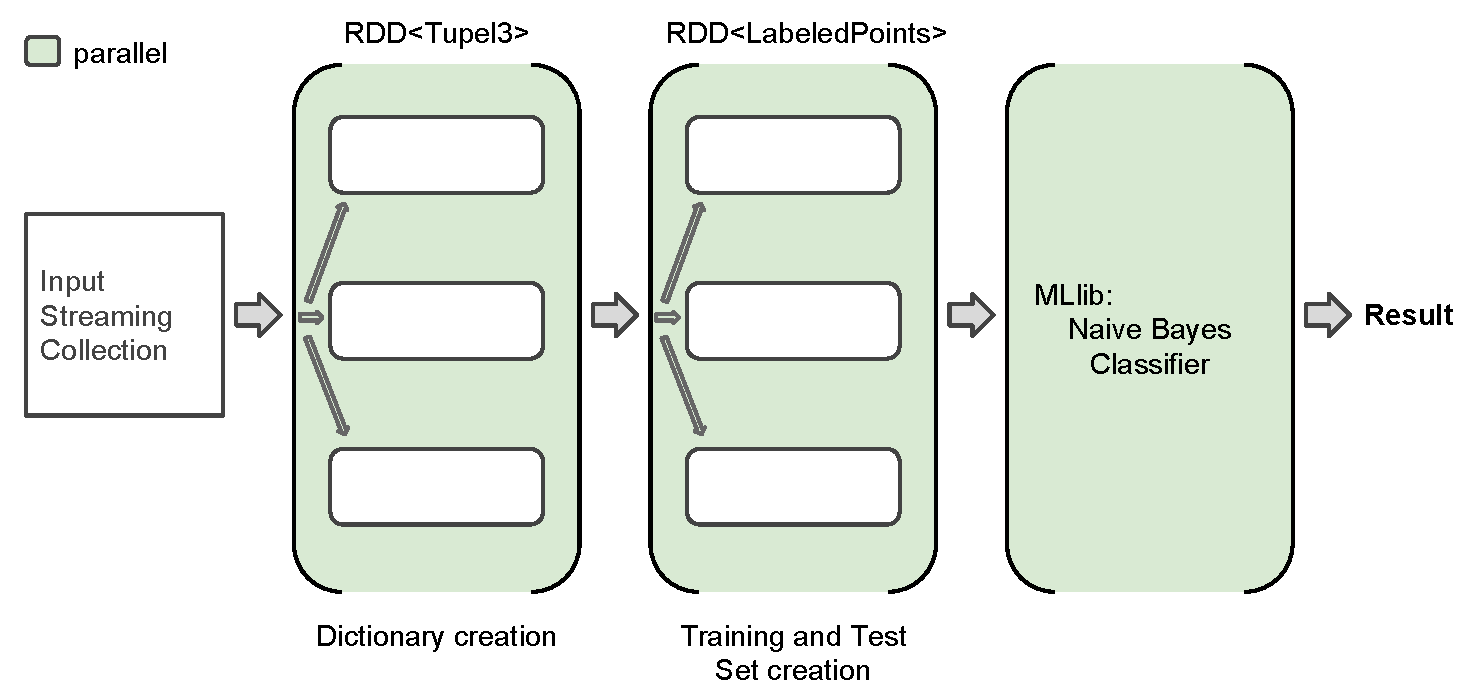
\includegraphics[scale=0.56]{VisualisationOfflineWorkflow.pdf}
%  \caption{Offline Workflow}
%\end{figure}

\subsection{Evaluation}
%write here
texttexttext

\subsection{Results}
%write here
texttexttext

\subsection{Summary}
%write here
texttexttext

\bibliographystyle{unsrt}
\small{
\bibliography{literatureDB}
}
\end{document}
